%\documentclass[12pt]{article}
\documentclass[12pt]{scrartcl}
\title{Assignment Template}
\nonstopmode
%\usepackage[utf-8]{inputenc}
\usepackage{lipsum}
\usepackage{graphicx} % Required for including pictures
\usepackage[figurename=Figure]{caption}
\usepackage{float}    % For tables and other floats
\usepackage{verbatim} % For comments and other
\usepackage{amsmath}  % For math
\usepackage{amssymb}  % For more math
\usepackage{fullpage} % Set margins and place page numbers at bottom center
\usepackage{paralist} % paragraph spacing
\usepackage{listings} % For source code
\usepackage{subfig}   % For subfigures
%\usepackage{physics}  % for simplified dv, and 
\usepackage{enumitem} % useful for itemization
\usepackage{siunitx}  % standardization of si units

\usepackage{tikz,bm} % Useful for drawing plots
%\usepackage{tikz-3dplot}
\usepackage{circuitikz}

%%% Colours used in field vectors and propagation direction
\definecolor{mycolor}{rgb}{1,0.2,0.3}
\definecolor{brightgreen}{rgb}{0.4, 1.0, 0.0}
\definecolor{britishracinggreen}{rgb}{0.0, 0.26, 0.15}
\definecolor{cadmiumgreen}{rgb}{0.0, 0.42, 0.24}
\definecolor{ceruleanblue}{rgb}{0.16, 0.32, 0.75}
\definecolor{darkelectricblue}{rgb}{0.33, 0.41, 0.47}
\definecolor{darkpowderblue}{rgb}{0.0, 0.2, 0.6}
\definecolor{darktangerine}{rgb}{1.0, 0.66, 0.07}
\definecolor{emerald}{rgb}{0.31, 0.78, 0.47}
\definecolor{palatinatepurple}{rgb}{0.41, 0.16, 0.38}
\definecolor{pastelviolet}{rgb}{0.8, 0.6, 0.79}
\begin{document}

\noindent
\begin{minipage}{0.15\textwidth}
    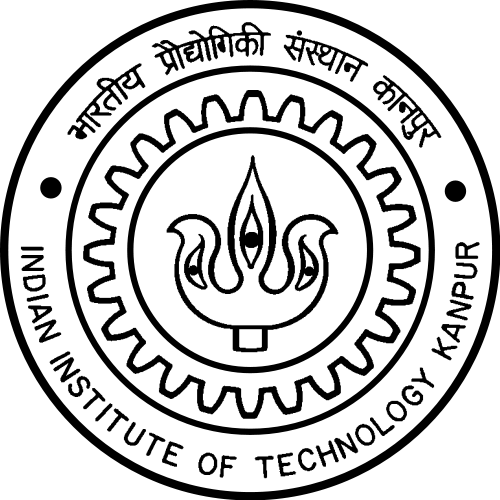
\includegraphics[width=\linewidth]{logo_black.png}
\end{minipage}%
\hfill
\begin{minipage}{0.8\textwidth}
    \begin{center}
        {\textbf{\Large Indian Institute of Technology Kanpur}} \\ \vspace{5pt}
        {\textbf{CGS698C --- Bayesian Models and Data Analysis}}
    \end{center}
\end{minipage}

\vspace{0.4cm}
\hrule
\vspace{0.4cm}
{\hspace{-11.5pt}\textbf{Name:}\ Anandan Iyer \hspace{\fill} \textbf{Due Date:} $19^{\text{th}}$ February 2026, 11:59 PM\\
{\textbf{Roll Number:}}\ 240117 \hspace{\fill} \textbf{Assignment:} 3\\
{\textbf{Department:}}\ Mechanical Engineering \\
\hrule

\paragraph*{Problem 1}
\textbf{Using Bayes’ theorem for statistical inference I}
\paragraph*{Exercise 1.4.1}
\textbf{Estimate the posterior density for the following values of $\theta$.}
\begin{itemize}
    \item $\theta = 0.75$
    \item $\theta = 0.25$
    \item $\theta = 1$
\end{itemize}
\textbf{Solution: } \\
    \begin{align*}
        L(\theta | y=7) &= \frac{10!}{7! (10-7)!} \theta^7 (1-\theta)^3 = 120 \theta^7 (1-\theta)^3 \\
        \therefore p(\theta | y=7) &= \frac{120 \cdot \theta^7 (1-\theta)^3 \times 2}{227 / 1408} = \frac{337920}{227} \theta^7 (1-\theta)^3
    \end{align*}
    \[
    p(\theta | y=7) = 
    \begin{cases} 
        \frac{337920}{227} \theta^7 (1-\theta)^3 & ; \ 0.5 \le \theta \le 1 \\ 
        0 & ; \ \theta < 0.5 \text{ or } \theta > 1 
    \end{cases}
    \]
    For $\theta = 0.75$:
    \begin{align*}
        p(\theta=0.75) &= \frac{337920}{227} \times (0.75)^7 (0.25)^3 \simeq 3.104
        \end{align*}
    For $\theta = 0.25$:
    \begin{align*}
        p(\theta=0.25) &= 0 
        \end{align*}
    For $\theta = 1$:
    \begin{align*}
        p(\theta=1) &= \frac{337920}{227} (1)^7 (1-1)^3 = 0
    \end{align*}
\newpage
\paragraph*{Exercise 1.4.2}
\textbf{Graph the posterior distribution of $\theta$.(Hint: Create a vector containing a lot of equidistant values of $\theta$ between say 0 and 1;
calculate posterior density for each value in the vector; plot a graph with values of $\theta$ on
the x-axis and associated posterior densities $p(\theta|y)$ on the y-axis.)} \\ \\
\textbf{Solution :}
    \begin{figure}[H]
        \centering
        
\includegraphics[width=0.8\linewidth]{Figure_1.png}
        \caption{Posterior Distribution of $\theta$ values spaced at equal intervals}
        \label{fig:Posterior Distribution of $\theta$ values spaced at equal intervals}
    \end{figure}

\paragraph*{Exercise 1.4.3}
\textbf{What value of $\theta$ has the maximum posterior density?} \\ \\
\textbf{Solution :} \\
Let's define a function $f(\theta)$, optimizing which, we would obtain the value(s) of $\theta$ where the function is maximized. 
    \begin{align*}
        f(\theta) &:= \theta^7 (1-\theta)^3 \\
        f'(\theta) &= 7\theta^6(1-\theta)^3 - 3\theta^7(1-\theta)^2 \\
        &= \theta^6(1-\theta)^2 \{7(1-\theta) - 3\theta\} \\
        &= \theta^6(1-\theta)^2 \{7 - 10\theta\}
    \end{align*}
    At the optimal value, $f'(\theta) = 0 \Rightarrow \theta^6(1-\theta)^2(7 - 10\theta) = 0$
    \[ \Rightarrow \theta = 0 \text{ or } 1 \text{ or } \frac{7}{10} \]
    Note : At $\theta = 1$ or 0, $f(\theta) = 0$. However at at $\theta = 0.7$, $f(\theta) > 0$. $\therefore$ at $\theta = 0.7$, $f(\theta)$ obtains a local maxima. Hence, the posterior density is maxmized when $\theta = 0.7 \Box$

\paragraph*{Exercise 1.4.4}
\textbf{Compare the graphs of the likelihood function, the prior distribution, and the posterior
distribution} \\ \\ 
\textbf{Solution :}
    \begin{figure}[H]
        \centering
        
\includegraphics[width=0.8\linewidth]{Figure_2.png}
        \caption{}
        \label{fig:figure_2}
    \end{figure}
    Comparison of the graph of the likelihood function, the prior and the posterior distribution.
    \begin{itemize}
        \item The prior distribution is a flat line from $0.5$ to $1$.
        \item The likelihood function is a continuous binomial curve that peaks at $0.7$.
        \item The posterior distribution resembles the product of the prior and the likelihood function.
    \end{itemize}
\newpage
\paragraph*{Problem 2} 
\textbf{Model building in the Bayesian framework}

\paragraph*{Exercise 2.5.1} 
\textbf{Graph the unnormalized posterior distribution of $\mu$ for the Null hypothesis model.}\\ \\
\textbf{Solution :} \\
\begin{figure}[H]
        \centering
        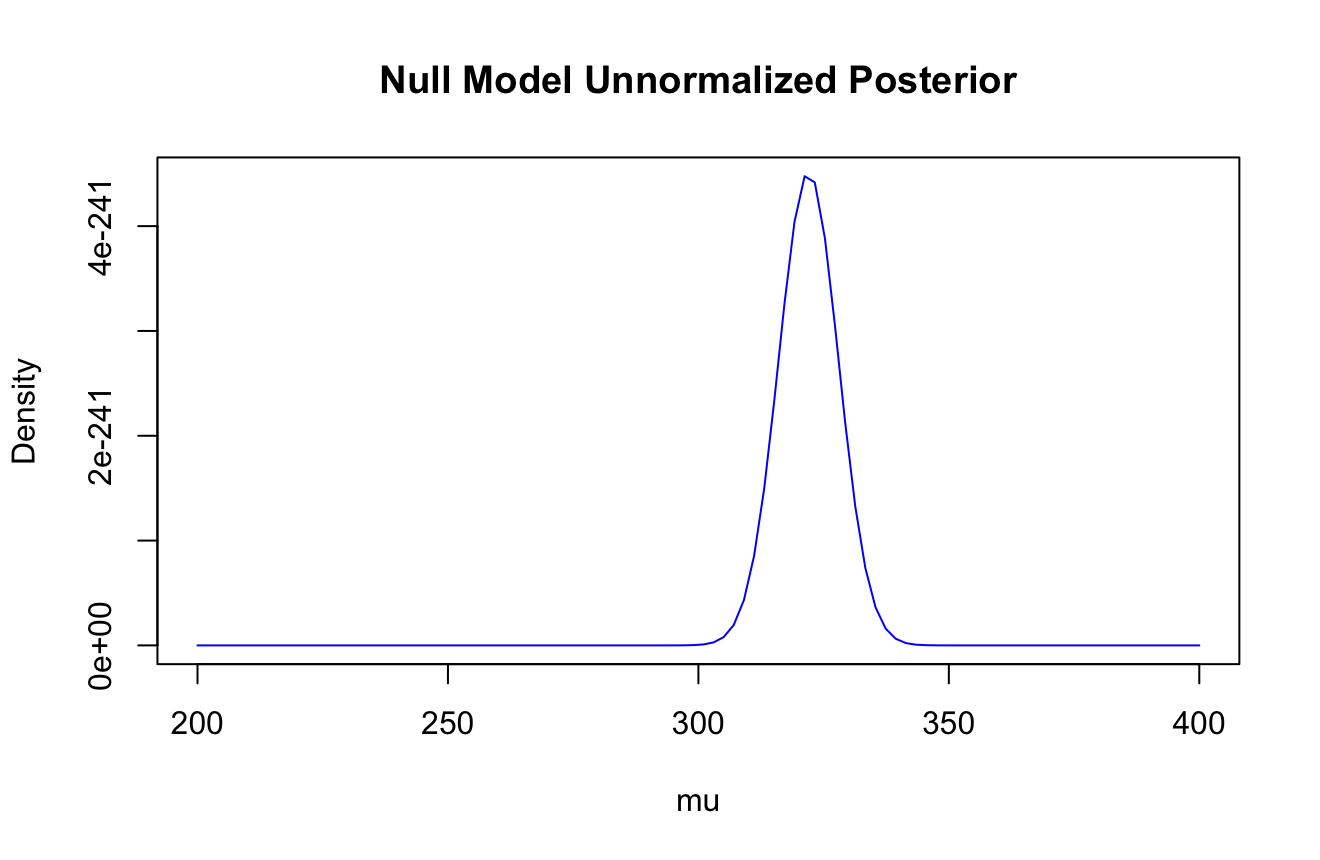
\includegraphics[width=0.6\linewidth]{Figure_3.png}
        \caption{Unnormalized posterior distribution of $\mu$ for the Null hypothesis model.}
        \label{fig:Unormalized posterior distribution of µ for the Null hypothesis model.}
    \end{figure}
\paragraph*{Exercise 2.5.2}
\textbf{Generate the prior predictions from the lexical-access model.} \\
\textbf{Solution :}
\begin{figure}[H]
        \centering
        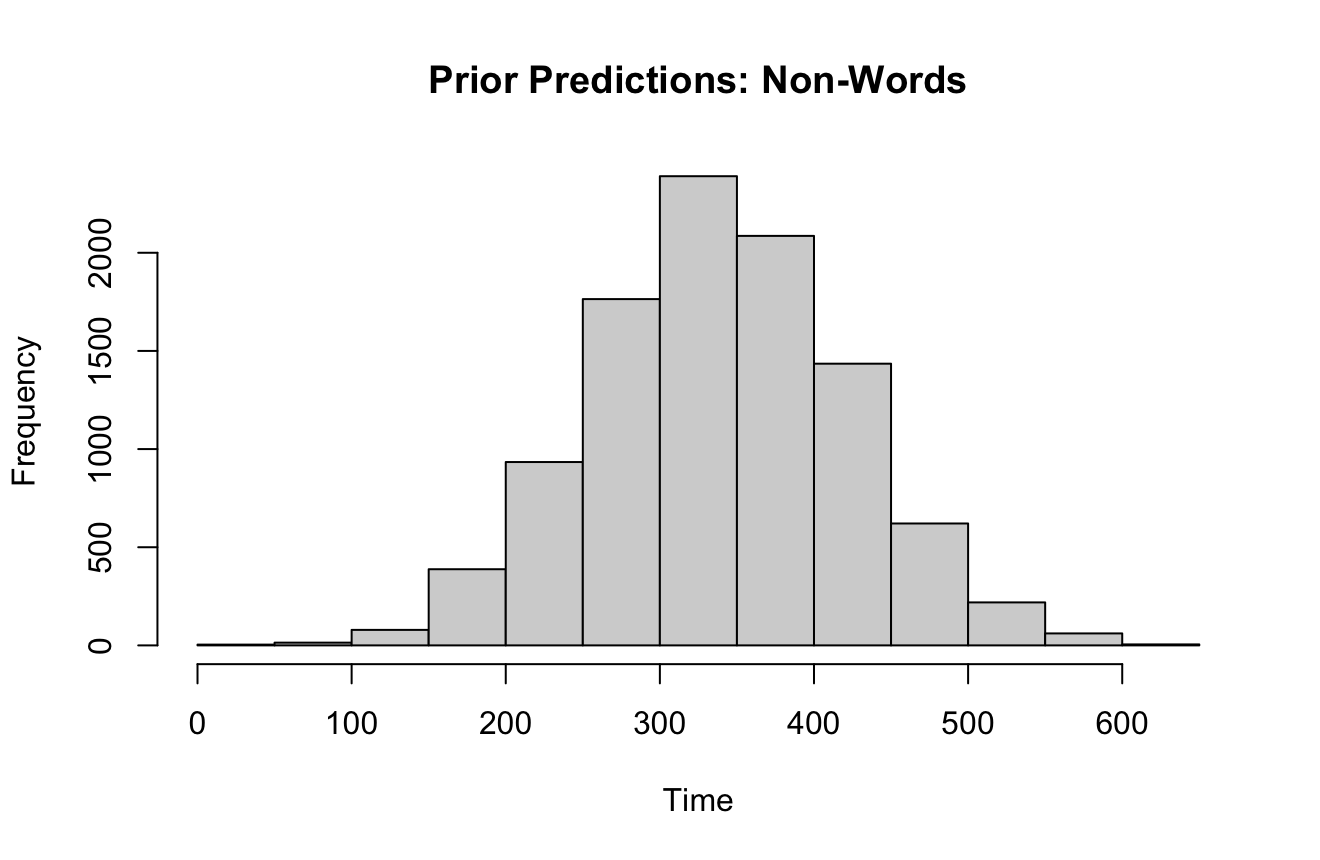
\includegraphics[width=0.6\linewidth]{Figure_4.png}
        \caption{Prior predictions from the lexical-access model.}
        \label{fig:Unormalized posterior distribution of µ for the Null hypothesis model.}
    \end{figure}
\newpage
\paragraph*{Exercise 2.5.3}
\textbf{Compare the prior predictions of the null hypothesis model and the lexical access model.}\\ \\
\textbf{Solution :} \\
\begin{figure}[H]
        \centering
        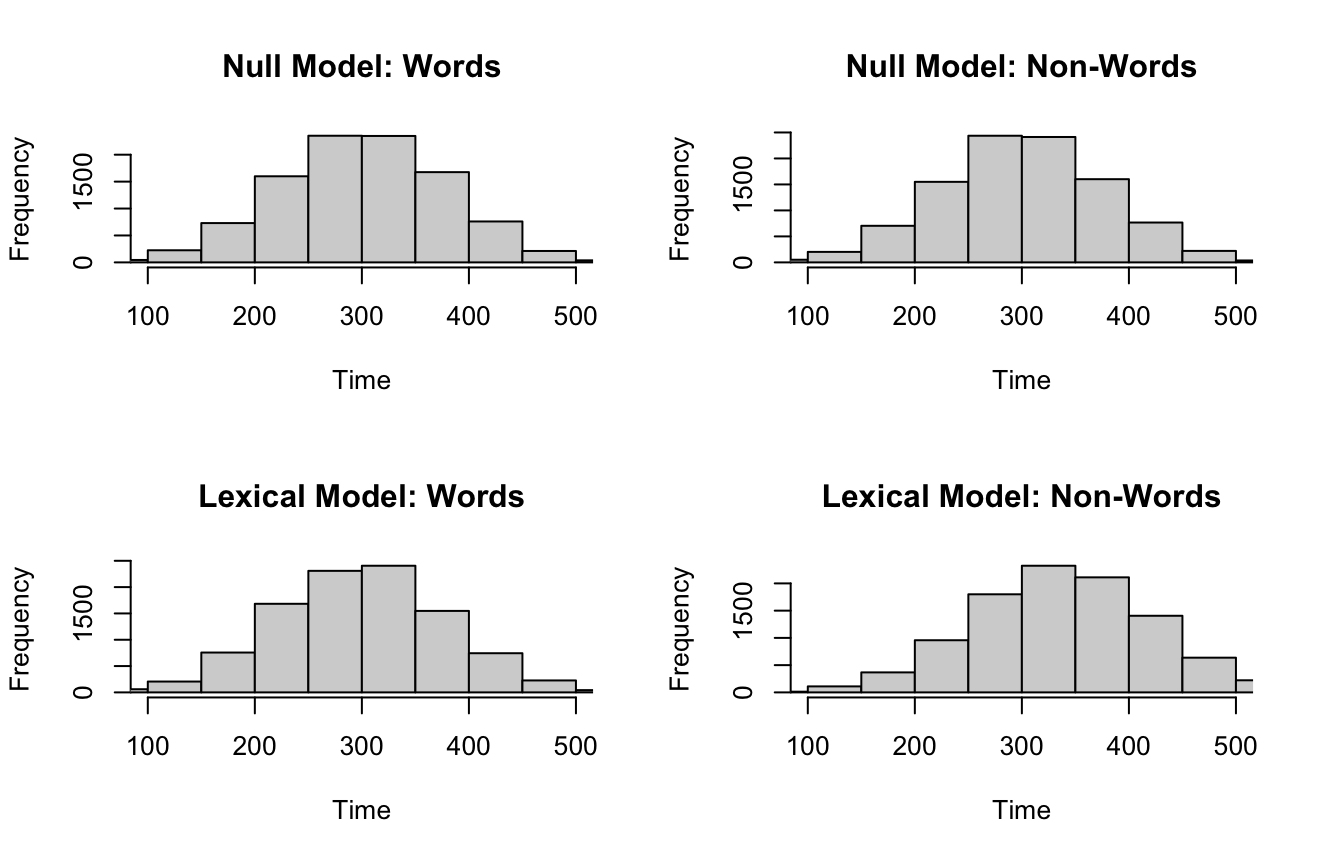
\includegraphics[width=0.6\linewidth]{Figure_5.png}
        \caption{Comparison of the Prior Predictions of the Null Hypothesis Modela and the Lexical Access Model}
        \label{fig:Unormalized posterior distribution of µ for the Null hypothesis model.}
    \end{figure}
\paragraph*{Exercise 2.5.4}
\textbf{Compare the prior predictions of each model against the observed data $T_w$ and $T_{nw}$.
Which model seems more consistent with the data?}\\
\textbf{Solution :} \\
\begin{figure}[H]
        \centering
        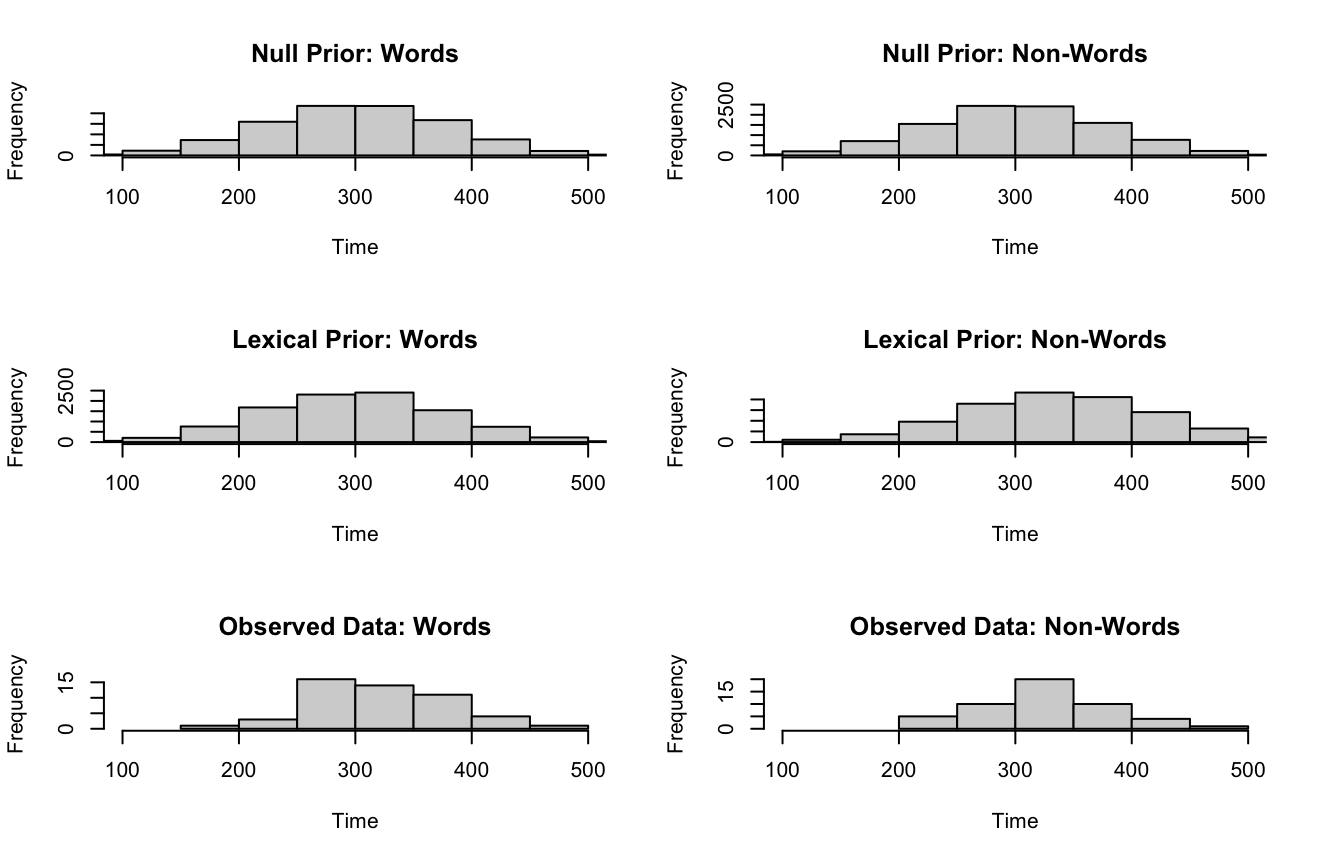
\includegraphics[width=0.6\linewidth]{Figure_6.png}
        \caption{Comparison of the Prior Predictions of each Model against the observed data $T_w$ and $T_{nw}$}
        \label{fig:Unormalized posterior distribution of µ for the Null hypothesis model.}
    \end{figure}
$\therefore$ The \textbf{Lexical-Access Model} is more consistent with the data. The Null Hypothesis model incorrectly predicts no difference between the two distributions.
\paragraph*{Exercise 2.5.5}
\textbf{Graph the unnormalized posterior distribution of $\delta$ for the lexical-access model.}\\ \\
\textbf{Solution :} \\
\begin{figure}[H]
        \centering
        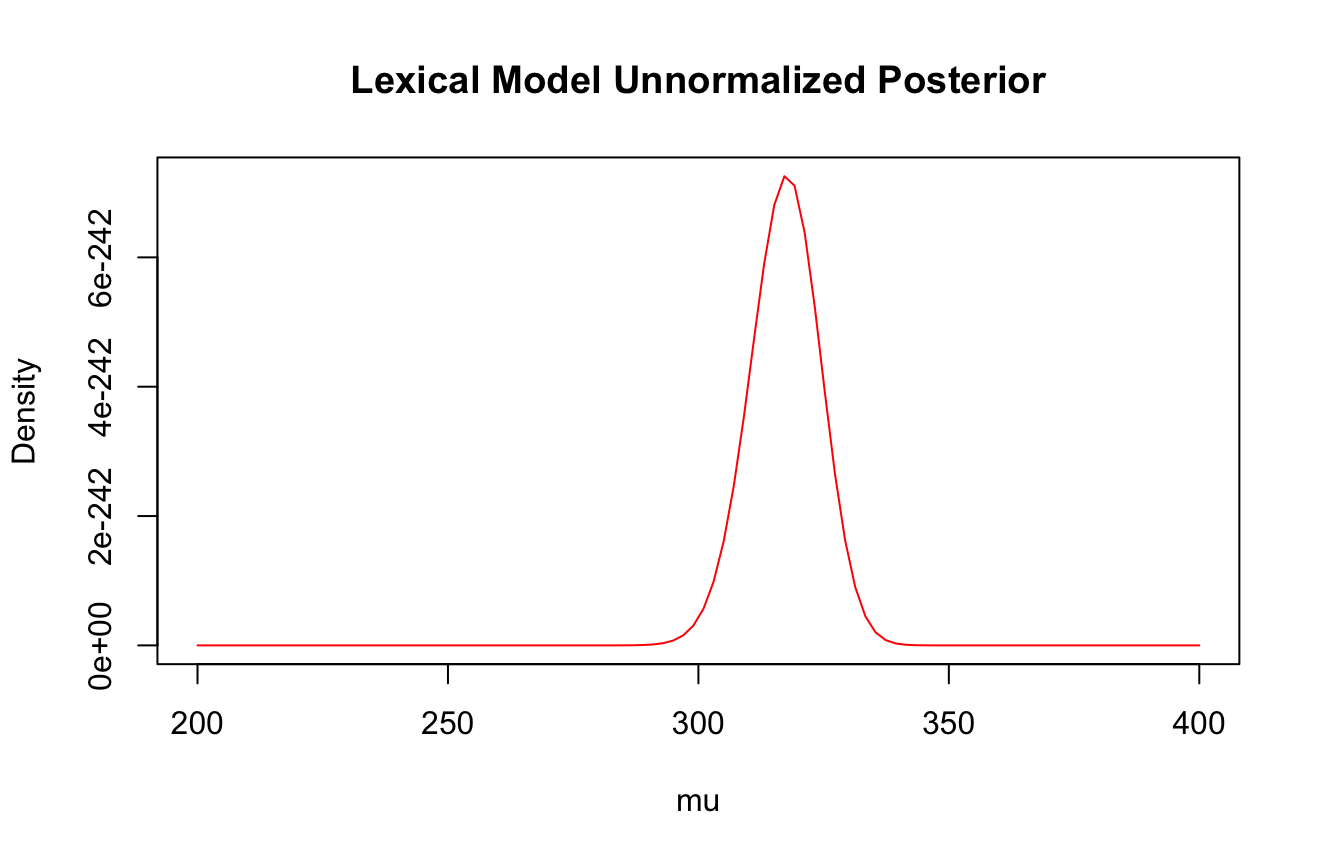
\includegraphics[width=0.6\linewidth]{Figure_7.png}
        \caption{Unnormalized posterior distribution of $\delta$ for the Lexical-Access model.}
        \label{fig:Unormalized posterior distribution of µ for the Null hypothesis model.}
    \end{figure}
\end{document}